\documentclass{article}
\usepackage[ngerman]{babel}
\usepackage[T1]{fontenc}
\usepackage[utf8x]{inputenc}
\usepackage{graphicx}
\usepackage{spreadtab}
\usepackage{booktabs}
\usepackage{hyperref}
\usepackage[left=25mm,right=25mm,top=25mm,bottom=25mm]{geometry}

\title{Pflichtenheft}
\date{\today}
\author{Projekt 3 EIT, Team 2: Reto Freivogel, Alexander Murray, Raphael Frey}

\begin{document}
\maketitle

\section{L\"osungskonzept}
\begin{figure}[h!]
    \begin{centering}
    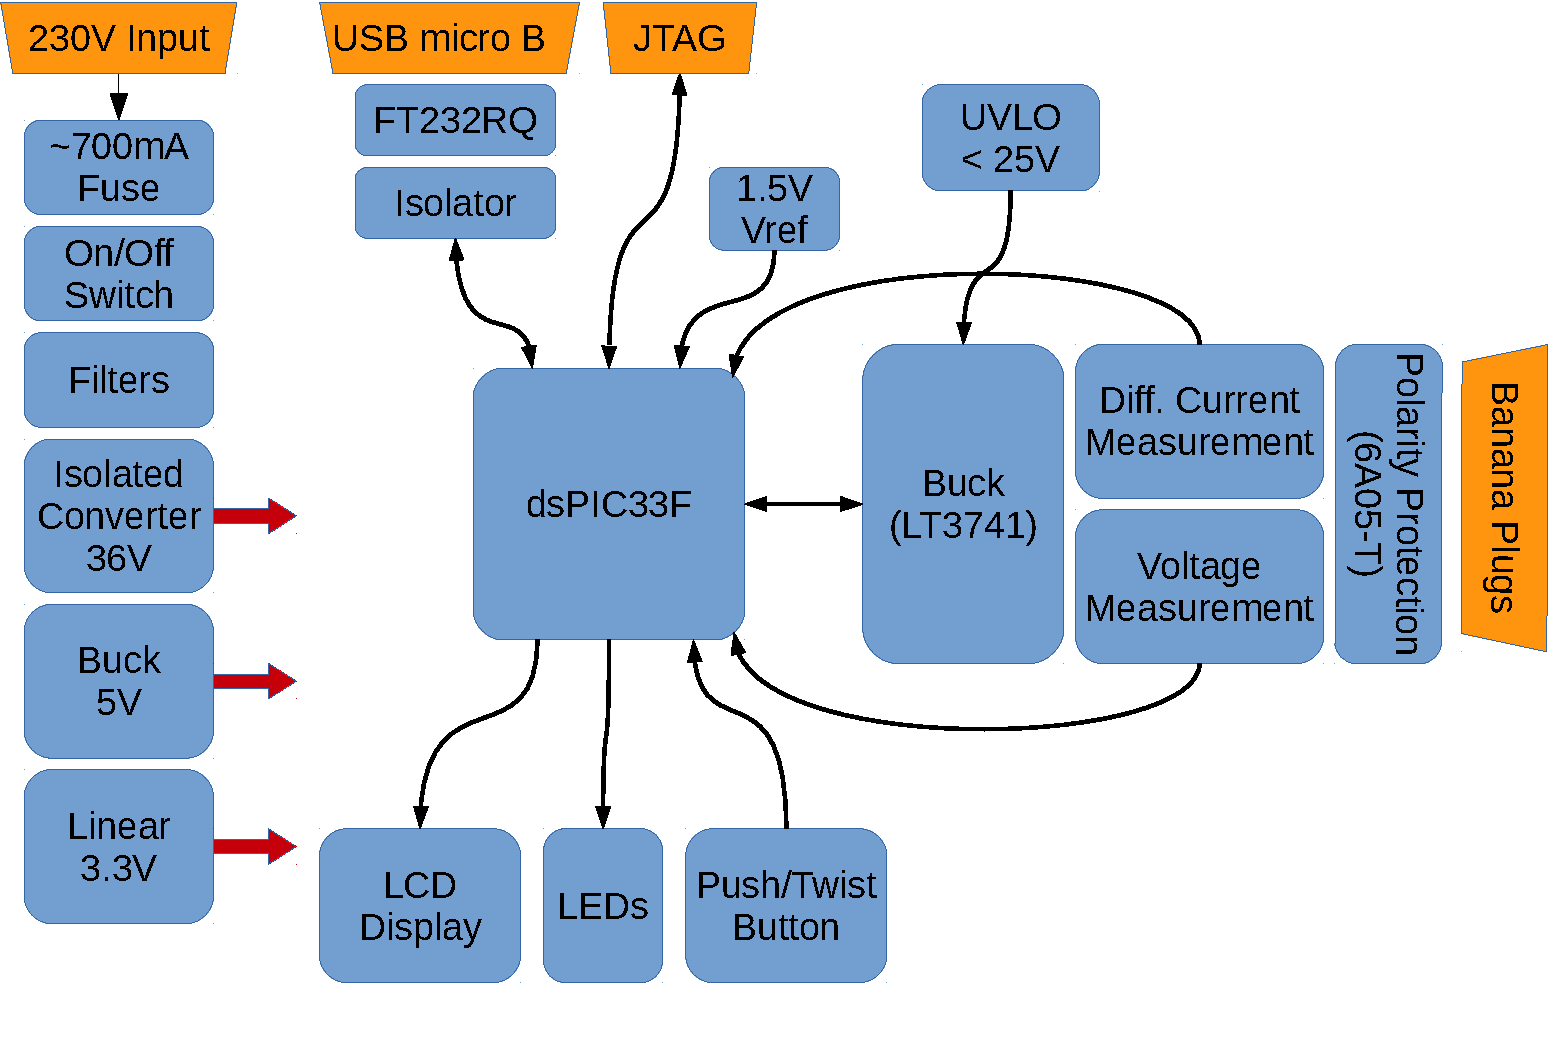
\includegraphics[width=.667\textwidth]{grob-blockdiagramm.pdf}
    \caption{Blockdiagramm des L\"osungsansatzes}
    \end{centering}
    \label{fig:grob-blockschaltbild}
\end{figure}

Das Kernst\"uck des Ger\"ates besteht  aus dem CVCC (Constant Voltage Constant
Current) Spannungswandler  und dem Mikrocontroller. Der  Mikrocontroller misst
differentiell Ausgangsstrom  und Single-Ended Ausgangsspannung  anhand seiner
eingebauten $ADC$s und  kann  somit   durch  zwei $DAC$s die  Spannungs-   und
Stromlimite  des  Wandlers einstellen  beziehungsweise regeln. Damit  bildet
er  die I-V  Kennlinie eines PV-Moduls nach.

Neben den Ausgangsspannungs- und Ausgangsstromanforderungen und dynamisch
einstellbare Strombegrenzung ist einer der wichtigsten Eigenschaften des
Spannungswandlers die F\"ahigkeit, Strom aufnehmen zu k\"onnen, im Falle dass
der Ausgang in Serie mit anderen Simulatoren h\"angt. Der LT3741 von Linear
erf\"ullt alle Anforderungen und wird in diesem Projekt verwendet.

Der LT3741 arbeitet mit Steuerspannungen im Bereich von $0V$ bis $1.5V$. Damit
die h\"ochstm\"oglichste Aufl\"osung der $ADC$s und $DAC$s erzielt werden kann,
wird eine $1.5V$ Referenzspannung, ersichtlich in der Abbildung
\ref{fig:grob-blockschaltbild}, verwendet.

Die Ausgangsspannung ist mit Hilfe einer Diode Verpolungsgesch\"utzt, sprich,
die Kennlinie der Solarzelle geht nicht ins Negative, sondern flacht bei 0V
ab.

Der LT3741 kann per Software ein- oder ausgeschalten werden, und wird
zus\"atzlich (mit Vorrang) in Hardware ausgeschaltet falls die
$36V$-Speisung unter ca. $25V$ f\"allt. Das erlaubt ein kontrolliertes und
Vorhersehbares Verhalten des Spannungswandlers w\"ahrend Ein- und
Ausschaltvorg\"angen des Endproduktes.

Die Solarzelle wird mit folgender Formel modelliert:
\begin{equation}
I_d = I_{sc} \cdot \left(\frac{G}{G_0} - exp\left(\frac{V_d-V_{oc}}{V_t}\right)\right)
\end{equation}

Wobei   $I_{d}$   der   momentane  Strom,   $I_{sc}$   der   Kurzschlussstrom,
$\frac{G}{G_0}$    das   Beleuchtungsverh\"altnis,    $V_d$   die    momentane
Ausgangsspannung, $V_{oc}$  die Leerlaufspannung und $V_t$  die Dunkelspannung
aller Zellen in Serie sind. Der Einfluss der Temperatur wird in dieser Formel
vernachl\"assigt und sie gilt lediglich falls $V_{oc} > 5 \cdot V_t$.

Das   Ger\"at  wird   \"uber  ein   Text-LCD  und   einen  Dreh-Dr\"uck-Taster
bedient. Weiter  ist  ein  Ein-Aus  Schalter vorgesehen. Auf  dem  LCD  werden
die  Werte der  momentanenen Spannung  und  des momentanen  Stromes sowie  die
eingestellte Belechtungsst\"arke angezeigt. Dreht man  den Drehtaster wird die
Beleuchtungsst\"arke ver\"andert. Durch  Dr\"ucken des Tasters gelangt  man in
Untermen\"us,  in denen  man  die anderen  Parameter  ($I_{sc}$, $V_{oc}$  und
$V_t$) ver\"andern kann.

Es wird ein galvanisch getrennter USB micro B Anschluss eingebaut um
Kommunikation mit einem externen Ger\"at zu erlauben. Zum Debuggen des Systems
wird diese Funktionalit\"at sehr n\"utzlich sein.


\section{Ziel-Spezifikationen}
\begin{center}
\begin{tabular}{lr}
    Maximale Ausgangsspannung	& 24V    \\
    Maximaler Ausgangsstrom		& 3.5A   \\
    Effizienz bei Volllast		& 80\%   \\
    Leistungsverbrauch Leerlauf	& 3W     \\
    Nachregelzeit				& 1ms    \\
    Genauikeit Spannung			& 2\%    \\
    Genauikeit Strom			& 2\%    \\
    Rippel Spannung				& 300mV  \\
    Rippel Strom				& 100mA  \\
    Stufen Kennlinie			& 3      \\
\end{tabular}
\end{center}

\section{Komponenten}

\begin{center}
\begin{spreadtab}{{tabular}{llrrr}}
    \toprule
    @ Digikey & @ Beschreibung & @ Preis & @ Anzahl & @ Betrag \\
    \midrule
    %1 & 2 & 3 & 4 & 5 \\
    @ DSPIC33EP16GS506-I/PT-ND & @ dsPIC33 microcontroller         & 4.91  & 1 & [-2,0] * [-1,0] \\
    @ 768-1008-1-ND            & @ FT232RQ (UART to serial)        & 4.5   & 1 & [-2,0] * [-1,0] \\
    @ NHD-0440WH-ATMI-JT\#-ND  & @ LCD Display, 80 (4x20) chars    & 24.9  & 1 & [-2,0] * [-1,0] \\
    @ LT3741EUF\#PBF-ND        & @ CVCC buck converter             & 8.44  & 1 & [-2,0] * [-1,0] \\
    @ TBD                      & @ MOSFET                          & 5     & 2 & [-2,0] * [-1,0] \\
    @ 285-1829-ND              & @ ACDC 230V to 36V supply module  & 27.41 & 1 & [-2,0] * [-1,0] \\
    @ J151-ND                  & @ Banana Plugs                    & 0.70  & 2 & [-2,0] * [-1,0] \\
    @ TBD                      & @ Twistbutton                     & 10    & 1 & [-2,0] * [-1,0] \\
    @ TBD                      & @ Misc. components                & 40    & 1 & [-2,0] * [-1,0] \\
    \midrule
    @ \textbf{Subtotal}        & @                                 & @     & @ & sum(e2:e10)     \\
    \midrule
    @ Jackaltac                & @ Printed Circuit Board           & 40    & 1 & [-2,0] * [-1,0] \\
    @ TBD                      & @ Housing                         & 40    & 1 & [-2,0] * [-1,0] \\
    \midrule
    @ \textbf{Subtotal}        & @                                 & @     & @ & sum(e11:e13)    \\
    \bottomrule
\end{spreadtab}
\end{center}

\section{Testkonzept}

\begin{itemize}
    \item
        Testen der oben angegebenen Spezifikationen.
    \item
        Verhalten  von  Strom  und   Spannung  bei  verschiedenen  resistiven,
        kapazitiven und induktiven Lasten (und Kombinationen davon).
    \item
        Verhalten von  Floating Potential und Stromaufnahme  bei verschiedenen
        resistiven,  kapazitiven  und  induktiven  Lasten  (und  Kombinationen
        davon).
    \item
        Verifikation  der korrekten  Funktionsweise  des Interfaces  (Display,
        Drehknopf).
\end{itemize}
\end{document}
